\apendice{Manual de especificación de diseño}
En este anexo se propone la realización de los diagramas de despliegue correspondientes al desarrollo del proyecto.

No se ha realizado ningún diagrama de despliegue específico para ninguna de las versiones propuestas puesto que no se ha llegado a crear la aplicación móvil de interacción de usuario-prototipo y tampoco se han definido clases en los programas de Arduino\cite{ArduinoIDE} creados para cada una de las versiones. 

Sin embargo, se ha creado un diagrama común para la visualización de las funciones, atributos y nodos correspondientes a los prototipos. Se pueden ver las distintas funciones y atributos en el diagrama \ref{fig:digDespliegue}:

% Inicio de la figura
\begin{figure}[h]
    \centering
    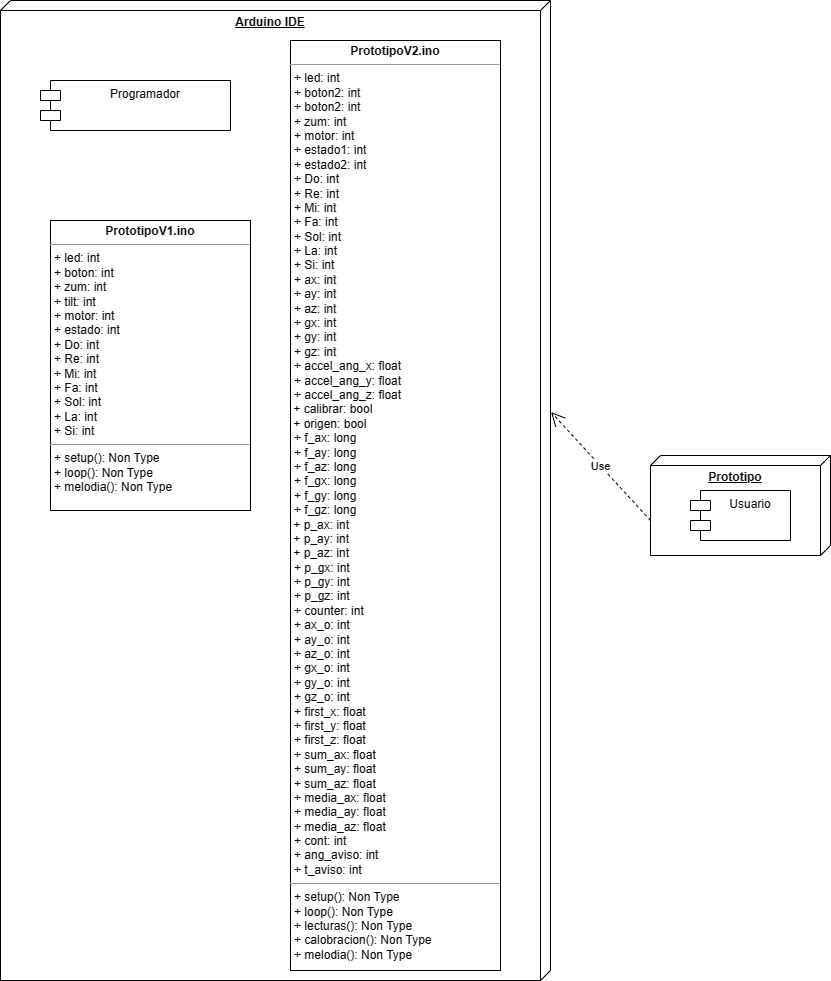
\includegraphics[width=0.8\textwidth]{img/DiagramDespliegue.png}
    \caption{Diagrama de los programas de los prototipos. Fuente propia.}
    \label{fig:digDespliegue} 
\end{figure}


